\section{Analysis}
\label{sec:analysis}
\FloatBarrier
\suppressfloats[t]

This section analyzes why \systemname{} works and its broader application. We first isolate its three core design choices under a shared trace pool and execution harness (\cref{sec:analysis:core_design}), then characterize the standard operating procedures it distills (\cref{sec:analysis:sops}), study how patch value composes (\cref{sec:analysis:selective_patch_aggregation}), and test transfer in broader real-world tasks (\cref{sec:analysis:broader_application}).

\subsection{Core Design Comparisons}
\label{sec:analysis:core_design}

\systemname{} rests on three design choices, which we isolate here by comparing each against its natural alternative under the same trace pool and execution harness: parallel many-to-one consolidation versus sequential editing (speed without quality loss), a single consolidated skill versus experience memory retrieval (reuse without test-time retrieval), and agentic versus single-call error analysis (more accurate root-cause patches).

\begin{table}[H]
\centering
\centering
\small
\setlength{\tabcolsep}{4pt}
\caption{Parallel consolidation versus sequential editing on SpreadsheetBench (same trace pool, +Error). Parallel outperforms Seq in effectiveness and efficiency. \cref{tab:math_seq_parallel} and \cref{tab:vqa_seq_parallel} show similar trend in math/VQA.}
\label{tab:seq_parallel}
\begin{tabular}{@{}l ccc ccc c@{}}
\toprule
& \multicolumn{3}{c}{\textit{Skill User: 122B}}
& \multicolumn{3}{c}{\textit{Skill User: 35B}} & \\
\cmidrule(lr){2-4}\cmidrule(lr){5-7}
\textbf{Condition}
    & \textbf{Vrf}$\uparrow$ & \textbf{Soft}$\uparrow$ & \textbf{Hard}$\uparrow$
    & \textbf{Vrf}$\uparrow$ & \textbf{Soft}$\uparrow$ & \textbf{Hard}$\uparrow$
    & \textbf{Time}$\downarrow$ \\
\midrule
Seq-$B{=}4$           & 59.00 & 40.63 & 20.63 & 26.17 & 22.37 &  7.47 & $\sim$15 min \\
Seq-$B{=}1$           & 61.83 & 44.40 & 25.40 & 26.00 & \textbf{23.83} & \textbf{10.57} & $\sim$60 min \\
Parallel (ours)        & \textbf{65.83} & \textbf{46.60} & \textbf{27.43} & \textbf{27.00} & 22.20 &  8.20 & \textbf{$\sim$3 min} \\
\bottomrule
\end{tabular}

\end{table}

\myparagraph{Parallel Consolidation.}
Online skill evolution typically edits the skill as trajectory batches arrive, so later analyses depend on earlier edits.
We isolate the effect of our parallel many-to-one consolidation by comparing against two sequential baselines: Seq-$B{=}1$, which updates after every trajectory, and Seq-$B{=}4$, which updates after every four trajectories.
All conditions use error analysts only and initialize from the Human-Written skill.
\Cref{tab:seq_parallel} reports the resulting quality and wall-clock tradeoff.


Parallel consolidation is better on all 122B SpreadsheetBench metrics and on 35B Vrf; the exception is that Seq-$B{=}1$ is modestly higher on 35B Soft and Hard.
This small quality tradeoff comes with a large efficiency gap: parallel produces the skill in about 3~min, compared with 15~min for Seq-$B{=}4$ and 60~min for Seq-$B{=}1$.
Math reasoning and DocVQA show the same broad trend that parallel consolidation preserves or improves quality while being much faster; \cref{app:parallel_consolidation_details} gives the latency analysis and similar comparisons on math/VQA.



\Needspace{0.40\textheight}
\myparagraph{Holistic Skill vs.\ Retrieval.}
Past-experience retrieval is a common paradigm for reusing agent trajectories: experience-memory systems store reflections, memories, or procedural lessons from previous executions and retrieve relevant items at inference time \citep{shinn2023reflexionlanguageagentsverbal,wang2023voyageropenendedembodiedagent,ouyang2026reasoningbankscalingagentselfevolving,fang2026mempexploringagentprocedural,wang2024agentworkflowmemory,liu2025contextualexperiencereplayselfimprovement}.

\begin{wraptable}{r}{0.50\linewidth}
\centering
\centering
\small
\setlength{\tabcolsep}{4pt}
\caption{\systemname{} outperforms ReasoningBank-style retrieval on SpreadsheetBench (same trajectory pool). \cref{tab:math_retrieval} and \cref{tab:vqa_retrieval} show similar trend in math/VQA.}
\label{tab:reasoning_bank}
\begin{tabular}{@{}l l ccc@{}}
\toprule
\textbf{Setting}
    & \textbf{User}
    & \textbf{Vrf}$\uparrow$
    & \textbf{Soft}$\uparrow$
    & \textbf{Hard}$\uparrow$ \\
\midrule
\multirow{2}{*}{\makecell[l]{ReasoningBank\\\citep{ouyang2026reasoningbankscalingagentselfevolving}}}
    & 122B & 56.00 & 40.10 & 21.30 \\
    & 35B & 20.50 & 17.30 & 4.97 \\
\midrule
\multirow{2}{*}{\makecell[l]{Human-Written\\+Combined (ours)}}
    & 122B & \textbf{69.83} & \textbf{47.17} & \textbf{29.53} \\
    & 35B & \textbf{29.67} & \textbf{18.80} & \textbf{5.73} \\
\bottomrule
\end{tabular}

\end{wraptable}
We instantiate this paradigm with ReasoningBank \citep{ouyang2026reasoningbankscalingagentselfevolving}: following its original setting, we store lessons from both success and failure trajectories and retrieve the top-1 memory with Qwen3-Embedding-8B.
We compare it against +Combined, which uses the same trajectory pool. Results on same-model Deepening are shown in \cref{tab:reasoning_bank}. +Combined is consistently better than ReasoningBank.
This supports the advantage of consolidating trajectory evidence into a compact skill rather than retrieving isolated memories at test time. We exclude OOD evaluations, as retrieval is not applicable for WikiTQ and HiTab whose queries are too semantically distant from the queries of SpreadsheetBench.
% We attribute the gain to two factors: the skill integrates recurring lessons into the agent's standing instructions, while retrieval remains sensitive to surface similarity between the current query and stored memory keys.

\WFclear

\begin{figure}[t]
\centering
\begin{minipage}[t]{0.48\linewidth}
\centering
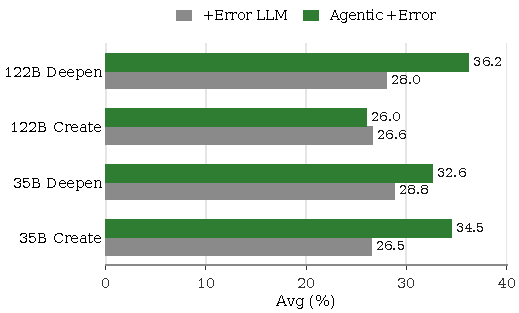
\includegraphics[width=0.86\linewidth,height=0.68\linewidth]{figures/fig_agentic_ablation_avg.pdf}
\caption{Agentic +Error versus single-call +Error~LLM on Avg, the balance of ID and OOD performance (same as Avg in \cref{tab:main_v1}). The agentic analyst inspects artifacts and validates fixes, whereas +Error~LLM reads only the execution log.}
\label{fig:agentic_ablation_avg}
\end{minipage}\hfill
\begin{minipage}[t]{0.48\linewidth}
\centering
\begingroup
\setlength{\columnwidth}{0.82\linewidth}%
\begin{tikzpicture}
\begin{axis}[
    width=\columnwidth,
    height=0.68\columnwidth,
    xmin=0, xmax=10,
    ymin=34, ymax=72,
    xlabel={Iteration},
    ylabel={SpreadsheetBench-Vrf (\%)},
    xtick={0,1,2,3,4,5,6,7,8,9,10},
    ytick={35,45,55,65},
    tick label style={font=\scriptsize},
    label style={font=\small},
    grid=major,
    grid style={black!8},
    axis line style={black!45},
    legend style={
        at={(0.5,-0.31)},
        anchor=north,
        draw=none,
        fill=none,
        font=\scriptsize,
        legend columns=2,
        /tikz/every even column/.append style={column sep=3pt}
    },
]
\addplot+[mark=o, thick, color=blue!70!black] coordinates {
    (0,48.33) (1,41.33) (2,40.83) (3,36.67) (4,44.33)
    (5,44.50) (6,49.50) (7,47.00) (8,52.83) (9,53.33) (10,55.17)
};
\addlegendentry{Greedy +Success}

\addplot+[mark=square*, thick, color=orange!85!black] coordinates {
    (0,48.33) (1,62.67) (2,64.17) (3,65.67) (4,65.17)
    (5,65.67) (6,60.83) (7,62.50) (8,62.67) (9,64.17) (10,63.33)
};
\addlegendentry{Greedy +Error}

\addplot+[mark=triangle*, thick, color=green!55!black] coordinates {
    (0,48.33) (1,56.83) (2,66.17) (3,62.50) (4,60.17)
    (5,62.17) (6,58.50) (7,59.00) (8,59.50) (9,59.17) (10,59.17)
};
\addlegendentry{Greedy +Combined}

\addplot+[no markers, dashed, very thick, color=blue!70!black] coordinates {
    (0,66.33) (10,66.33)
};
\addlegendentry{\systemname{} +Success}

\addplot+[no markers, dashed, very thick, color=orange!85!black] coordinates {
    (0,65.83) (10,65.83)
};
\addlegendentry{\systemname{} +Error}

\addplot+[no markers, dashed, very thick, color=green!55!black] coordinates {
    (0,69.83) (10,69.83)
};
\addlegendentry{\systemname{} +Combined}
\end{axis}
\end{tikzpicture}

\endgroup
\caption{Greedy selective patch aggregation on SpreadsheetBench-Vrf (pass rate, \%). Each curve adds one validation-selected patch per iteration ($x$-axis) from the Error, Success, or Combined pool; the flat line is full \systemname{} aggregation of all patches.}
\label{fig:greedy_patch_selection_vrf}
\end{minipage}
\end{figure}
\myparagraph{Agentic Error Analysis.}
Related work derives transferable lessons or skills from error trajectories via a single non-interactive LLM call \citep{ouyang2026reasoningbankscalingagentselfevolving,xia2026skillrlevolvingagentsrecursive,yang2026autoskillexperiencedrivenlifelonglearning,jiang2026xskillcontinuallearningexperience}. We ablate this design with \textbf{+Error~LLM}, where one LLM call reads each failed trajectory and proposes a patch without inspecting artifacts, querying ground truth, or validating fixes; \cref{fig:agentic_ablation_avg} compares it with our agentic error analyst. Agentic +Error achieves higher Avg than +Error~LLM in most settings, showing that interactive diagnosis is more useful than log-only patch generation; \cref{app:agentic_ablation_full} reports and discusses the full per-dataset results in \cref{tab:agentic_ablation}. The qualitative analysis in \cref{app:qual_agentic_vs_llm} shows the mechanism: artifact access and fix validation help the agentic analyst identify root causes more precisely.

\myparagraph{Apples-to-apples vs.\ head-to-head comparison.}
The above three comparisons are apples-to-apples, isolating each core design without the data, model, harness, and engineering confounders that complicate whole-system evaluation. As a complementary view, \cref{app:prior_systems} reports a direct head-to-head against three concurrent systems (XSkill \citep{jiang2026xskillcontinuallearningexperience}, EvoSkill \citep{alzubi2026evoskillautomatedskilldiscovery}, and SkillGen \citep{ma2026skillgenverifiedinferencetime}) under a shared open model and benchmark, where \systemname{} still shows its advantage.


\subsection{SoPs Learned}
\label{sec:analysis:sops}

Many-to-one merging keeps the operations that recur across trajectories and turns them into standard operating procedures (SoPs), rather than collecting one-off tricks.
Across the 323 map patches from the 122B Deepening +Combined run, four learned SoPs dominate, each cited by between $16\%$ and $55\%$ of patches (a single patch can cite more than one SoP), including: recalculating and reading back formulas after writes, verifying target cells before submitting, and deleting rows in a corruption-safe order.
Task-specific quirks are routed to on-demand \texttt{references/} files, keeping the SKILL.md focused on broadly reusable procedures (Details in \cref{app:sops}).

\subsection{Selective Patch Aggregation}
\label{sec:analysis:selective_patch_aggregation}

\systemname{} aggregates all learned patches into the target skill, avoiding the cost of per-patch validation. If patches vary in quality, can selecting a subset do better? We test two selectors against full aggregation: \textbf{greedy top-1}, which at each iteration adds the locally best patch according to validation on evolving set, and \textbf{Bayesian optimization (BO)}, which searches binary patch-inclusion vectors and reuses validation scores from previously tried subsets to bias later proposals toward promising combinations. Both use the 200-task evolving set (\cref{sec:experiments:main}) and a 32-task validation set from evolving set; \cref{app:selective_patch_aggregation} gives the full algorithmic details.

\myparagraph{Greedy rises quickly but plateaus below full aggregation.}
\cref{fig:greedy_patch_selection_vrf} shows greedy +Error and +Combined rising for a few iterations and then plateauing, with +Success dipping and only partially recovering; every greedy curve stays below full \systemname{} aggregation.
Two mechanisms drive the plateau (detailed in \cref{app:qual_patch_selection}).
(1) \emph{patch-irrelevant regression}: the patches flip some target tasks from wrong to correct, but their side effects also flip previously-correct tasks from correct to wrong, so net accuracy stalls.
(2) \emph{semantic overlap}: recurring errors lead the pipeline to propose patches that repeatedly target the same behaviors (e.g., formula recalculation, validation checklists), so a new patch largely restates existing guidance and adds little marginal gain.
Patch value is therefore combinatorial rather than a sum of singletons, which makes optimizing the combined effect of patches necessary.

\myparagraph{BO is useful but computationally heavy.}
BO searches patch subsets directly, so it can model complementarity and interference that greedy misses.
\cref{tab:bo_patch_selection} shows that, compared with applying all +Error patches, BO improves most selected metrics, especially the SpreadsheetBench columns.
The cost is validation: each candidate subset must be materialized as a skill and run on the validation set before it can inform the posterior, and larger patch universes increase this cost quickly.
We therefore view BO as useful when the target distribution and validation budget are known, rather than as a replacement for the default full aggregation in \systemname{}.

\begin{table}[t]
\centering
\setlength{\tabcolsep}{5pt}
\caption{BO-selected +Error patches versus applying all of them (No Selection), in the 122B Deepening spreadsheet setting. Evolve is the accuracy on evolving-set.}
\begin{tabular}{lcccccc}
\toprule
\textbf{Skill} & \textbf{Evolve} & \textbf{Vrf} & \textbf{Soft} & \textbf{Hard} & \textbf{WikiTQ} & \textbf{HiTab} \\
\midrule
No Selection (+Error) & 68.00 & 65.83 & 46.60 & 27.43 & 76.30 & \textbf{43.45} \\
BO Selection (+Error) & \textbf{72.83} & \textbf{69.83} & \textbf{47.27} & \textbf{28.90} & \textbf{77.51} & 43.38 \\
\bottomrule
\end{tabular}

\label{tab:bo_patch_selection}
\end{table}

\subsection{Broader Application}
\label{sec:analysis:broader_application}
We test broader application of \systemname{} in PDF extraction, PPTX editing, and DOCX editing. These settings use Anthropic's official \texttt{pdf}, \texttt{pptx}, and \texttt{docx} skills as starting points \citep{anthropic2026documentskills} and retain the same execution style as the spreadsheet experiments: agents operate over files with command-line tools and are scored by task-specific local verifiers.

Across the three domains, evolution on source traces improve performance on separate held-out targets. For PDF, VRDU traces transfer to VAREX, raising pass rate from 76.9\% to 85.3\% \citep{wang2023vrdu,barzelay2026varex}. For PPTX, TSBench traces transfer to a deck-disjoint TSBench OOD split, improving 72.5\% to 88.8\% \citep{jung2026talktoyourslides}. For DOCX, evolving on synthetic tasks that cover generic DOCX operations transfers to the OfficeBench DOCX subset, improving 79.7\% to 87.5\% \citep{wang2024officebench}. \cref{app:broader_application} provides setup and implementation details for each domain.
